\section{Capacity Constraints}
\label{sec:capacity}
Physical limitations to the size of hardware 
transactions are
governed by how they are implemented in hardware. 
Such capacity constraints
determine when a transaction will inevitably abort, 
even in the case of zero contention. We 
devised a parameterizable array access
experiment to measure the maximum cache line capacity 
of sequential read-only and write-only
hardware transactions. We also experimented with strided 
memory access patterns
to detect whether the read and write sets are maintained
on a per-cache line basis or a per-read / per-write basis.
With knowledge of the maximum sequential access 
capacity and also the maximum
strided access capacity, we can draw conclusions 
about where in the caching
architecture the read and write sets are 
maintained. 

\paragraph{Intel}
We experimentally support the hypothesis
that the Intel HTM implementation uses the L3 cache to 
store read sets and the L1 cache to store write sets.

\begin{figure}[h]
\centering
\begin{minipage}[b]{.45\linewidth}
\centering
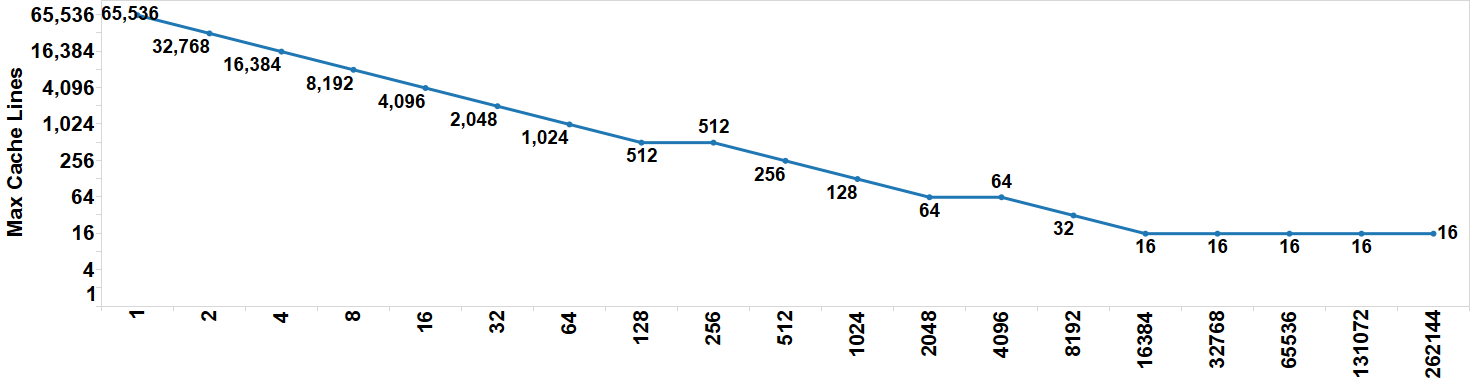
\includegraphics[width=\linewidth]{images/wttm_stride_read_intel}
\caption{$\log_2{\textrm{Stride}}$ vs $\log_2{\textrm{Lines Readable}}$.}
\label{fig:wttm_stride_read_intel}
\end{minipage}%
\quad
\begin{minipage}[b]{.45\linewidth}
\centering
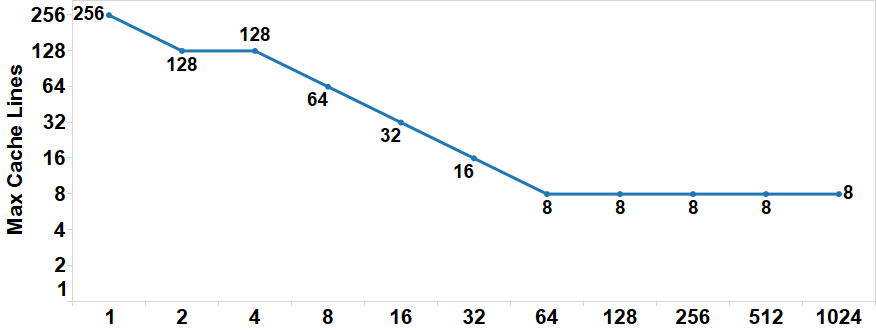
\includegraphics[width=\linewidth]{images/wttm_stride_write_intel}
\caption{$\log_2{\textrm{Stride}}$ vs $\log_2{\textrm{Lines Writable}}$.}
\label{fig:wttm_stride_write_intel}
\end{minipage}
\end{figure}

\figref{wttm_capacity_read_intel} summarizes the result of a sequential
read-only access experiment where data points represent the success
probability of the transaction with respect to the 
number of cache lines read.  We see that a 
single transaction can reliably read 
around 75,000 contiguous cache lines. 
The {L3} cache of the Intel machine has a maximum
capacity of $2^{17}$ ($=131,072$) cache lines and it is unlikely
for much more than half of the total capacity to 
fit perfectly into the {L3} due to
the hash function mapping physical address to L3 cache bank. 

\figref{wttm_stride_read_intel} shows the result of a strided read-only
access experiment. The stride amount indicates 
the number of cache lines per
iteration (e.g. reading cache lines 1, 5, 9, 13, 17 etc. 
indicates a stride of 4) and each data point 
represents the maximum number of cache
lines that can be reliably read with respect 
to the stride amount. For example,
the third data point in the graph indicates 
that when the stride amount is
$2^2$ ($=4$) (e.g. accessing every fourth cache line), 
the transaction can reliably read
$2^{14}$ ($=16,384$) cache lines and commit. 
We can see that the number of cache lines that can be 
read in a single transaction is generally
halved as we double the stride amount, presumably 
because the access pattern
accesses progressively fewer cache sets while 
completely skipping over the other sets.
It is important to note that the plot plateaus 
at $2^4$ ($=16$) cache lines.
When the stride amounts are large enough to consecutively
hit the same cache set we see support for 
the hypothesis that the read set is
maintained in the {L3} cache since the minimum number
of readable values never drops below 16, 
the L3 associativity.


% \figreftwo{wttm_capacity_read_intel}{wttm_stride_read_intel} show experimental results that indicate
% that the read set is maintained in the
% {L3} cache. The {L3} cache of this Intel machine has a maximum
% capacity of $2^{17}$ cache lines, which explains 
% why read-only transactions
% cannot fit much more than $2^{16}$ ($=65,536$) 
% cache lines because it is unlikely
% for the whole read set to fit perfectly into the {L3} due to
% the hash function mapping physical address to L3 cache bank. 
% The minimum of 16
% cache lines readable when the stride amounts 
% are large enough to consecutively
% hit the same cache set further supports the notion that the read set is
% maintained through the {L3} because this value exactly coincides 
% with the L3 associativity.

We also conducted similar experiments for write-only accesses
patterns.  \figref{wttm_capacity_write_intel} illustrates 
the result of an
identical array access experiment, except that the 
transactions are write-only
instead of read-only. A single write-only transaction 
can reliably commit about 400 contiguous cache lines. The
size of the {L1} cache is 512 cache lines and a transaction must also
have sufficient space to store other program metadata (e.g. the
head of the program stack), thus we would not expect to fill
all 512 lines perfectly.

\figref{wttm_stride_write_intel} illustrates that the number of cache
lines that can be written in a single transaction 
is also generally halved as we
double the stride amount.  However, even as we increase the stride amount
significantly, the number of cache lines that a 
transaction can reliably write
to does not fall below 8, corresponding to the associativity 
of the L1 cache.  This suggests that, at worst, one is limited 
to storing all writes in a single, but entire, set of the L1 cache.

\paragraph{IBM}
We experimentally support the hypothesis
that the IBM HTM implementation uses a dedicated structure
to maintain read and write sets, choosing not to extend the 
functionality of the existing cache structures as with
the Intel implementation.  In addition, we observe
that the dedicated structures used for read and write set
maintenance is not shared among the 8 threads per core, but rather
each thread is allocated its own copy.

\begin{figure}[h]%[ht!]
\centering
\begin{minipage}[b]{.45\linewidth}
\centering
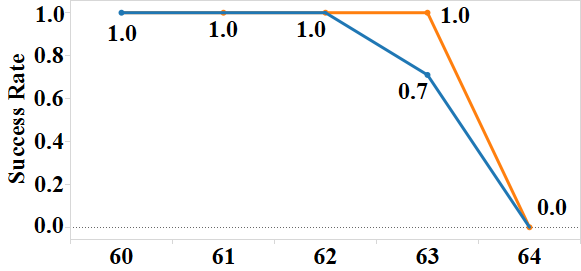
\includegraphics[width=\linewidth]{images/wttm_capacity_readwrite_ibm}
\caption{Lines Read/Written vs Success Rate.}
\label{fig:wttm_capacity_readwrite_ibm}
\end{minipage}%
\quad
\begin{minipage}[b]{.45\linewidth}%[ht!]
\centering
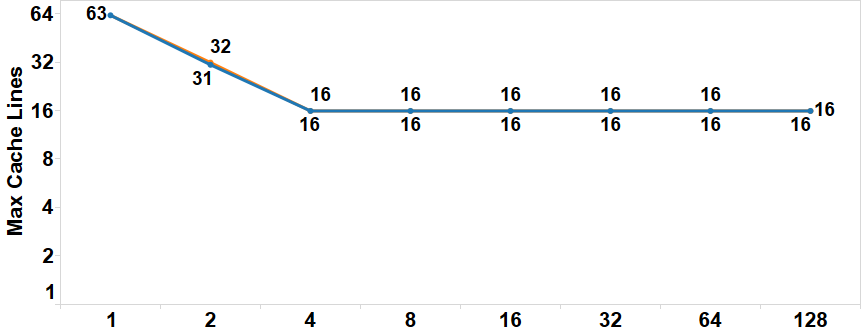
\includegraphics[width=\linewidth]{images/wttm_stride_readwrite_ibm}
\caption{Stride vs Lines Readable/Writeable.}
\label{fig:wttm_stride_readwrite_ibm}
\end{minipage}
\end{figure}


The results of our strided access experiment for 
both read-only and write-only
transactions appear to be identical in
\figref{wttm_stride_readwrite_ibm}, where
the maximum number of reads or writes in a transaction
is 64 and that the maximum transaction size 
halves as we double the stride amount with a minimum
of 16.  The maximum observed hardware transaction size is far too
small to be attributable to even the {L1} cache, which holds 512 cache
lines.   Thus, we conclude that there are dedicated caches 
for transactions in the IBM implementation independent
of the standard core caches, and that
these caches likely each have 4 sets and an associativity of 16.


A natural next question is whether this IBM machine 
has 10 dedicated caches that
are spread across each core, or if there are 80 
dedicated caches that are spread
across each hardware thread. To determine the 
difference, we experimented and
measured the number of successful write-only 
transactions that concurrently
running threads were able to complete. Each 
thread makes 10,000 transaction
attempts to write 40 thread-local cache 
lines and then commit. The
transaction size of 40 cache lines is designed 
to sufficiently fill up the
dedicated caches per transaction to induce capacity 
aborts in the case of shared
caches.

\begin{figure}[H]%[ht!]
\centering
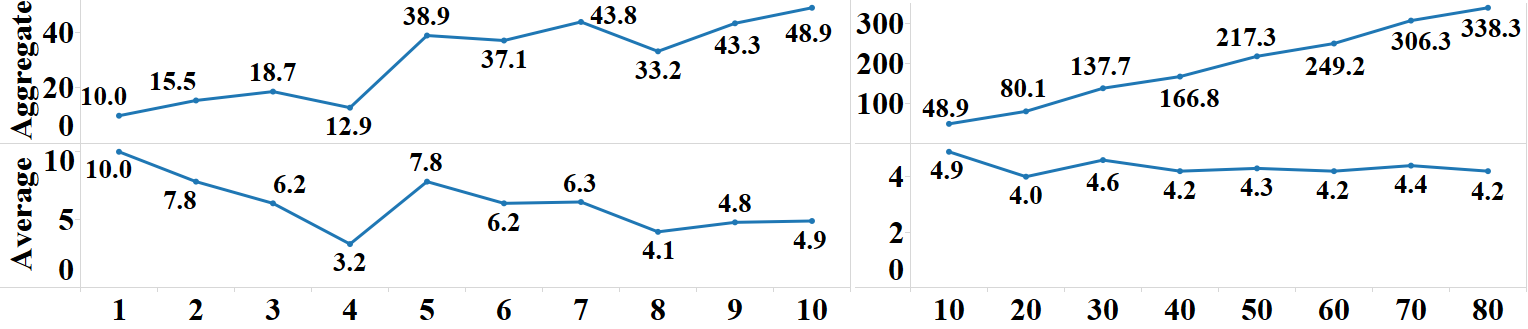
\includegraphics[width=\linewidth]{images/wttm_core_or_thread_ibm}
\caption{Number of Threads vs Committed Transactions (Thousands).}
\label{fig:wttm_core_or_thread_ibm}
\end{figure}


We see in \figref{wttm_core_or_thread_ibm} 
evidence that there are dedicated caches for each hardware 
thread and that they are not shared among
threads within a core. Each spawned
software thread is pinned to a unique hardware thread 
in round robin fashion
such that the distribution is even across the 10 cores. 
If all 8 of the
hardware threads on a single core share a single 
dedicated cache, we would
expect to see sublinear (or even no) speedup as we spawn
more running threads and assign them to the same core. 
Instead, we observe a
linear increase in the aggregate number of successfully 
committed transactions,
while the average per-thread number of successful 
transactions is constant.
Although the general 45\% success rate suggests some 
level of contention between
the running threads, it is most likely not due to 
per-core sharing of a
dedicated cache since the addition of other threads does
not decrease the aggregate throughput.
 



